This section of the document describes the major milestones of our project. It
is highly susceptible to change.

\subsection{Big Prototype Party (Monday, Oct 14th)}

\subsubsection*{Summary}
Since this project does not have a sponsor, the onus is on us to determine the
exact nature of the problem we would like to solve. To ensure that our efforts
are directed effectively for the remainder of our project, our first month has
been dedicated to researching and playtesting. By this date, every member of the
team should have a solid foundation of the problem space we are working in, and
have a prototype of a solution.

\subsubsection*{Deliverables}
Every member of the team must have a prototype of our final game. This prototype
should fit the following criteria:
\begin{itemize}
	\item The prototype is interactive.
	\item The prototype is engaging to work with.
	\item The prototype represents a wide slice of the game’s mechanics.
	\item The prototype makes the player think computationally.
	\item The rules of the prototype are concise and written out.
\end{itemize}

\subsection{Game Pitch (Friday, October 18th)}

\subsubsection*{Summary}
This milestone culminates one of the most critical stages of our project. Now
that we’ve had the time to demonstrate non-abstractly what our problem space is
and how we’d like to solve it, we can converge on a unified solution. By this
milestone the team should be able to confidently answer the following questions,
and develop the documentation necessary to capture our answers:
\begin{enumerate}
	\item What will our final product look like?
	\item What are the learning objectives of our game?
	\item What kind of puzzles will our game have?
	\item How will those puzzles work?
	\item How will those puzzles achieve our learning objectives?
	\item How will we order these puzzles to ensure that there is an appropriate
	learning curve?
	\item What evidence do we have that our learning curve will be engaging and
	effective for our target audience?
	\item What games did we draw inspiration from?
\end{enumerate}

\subsubsection*{Deliverables}
This milestone’s deliverables are still non-code items. These are items that we
will rely on for the remainder of our project, and inform all future efforts.
Specifically, we must deliver:
\begin{itemize}
	\item A unified prototype of our final game.
	\item A write up of our prototype, its capabilities, and its design philosophy.
	\item Diagrams/concept drawings of game mechanics not demonstrated by the prototype.
	\item Research Papers that support our design choices.
	\item Playtesting findings that support our design choices.
	\item Any other artifacts necessary to answer the questions above.
\end{itemize}

\subsection{Paper Prototype 2.0 (Monday, October 28th)}

\subsubsection*{Summary}
Rapid iteration is an important part of successfully designing a game. By this
milestone, our original prototype should be placed in the hands of as many
playtesters as possible. The group should use the data from this playtesting to
inform any design changes we make to our prototype.

\subsubsection*{Deliverables}
\begin{itemize}
	\item A new prototype of our final game, with documentation supporting our
	changes to our original prototype.
	\item Expanded design documentation to capture the vision of our final game
	including:
	\begin{itemize}
		\item Detailed system diagrams that describe how the mechanics of our game
		interact.
		\item An explanation of who will be the lead on certain areas of our game.
	\end{itemize}
\end{itemize}

\subsection{Hello Game (Friday, Dec 13th)}

\subsubsection*{Summary}
This milestone marks our the delivery of our proof of concept prototype. The teams' 
advisor will evaluate the prototype and provide recommendations for moving forward. 
The prototype will show an extremely basic vertical slice of our final game. 

\subsubsection*{Deliverables}
The only deliverable for this milestone will be the Hello World prototype. This prototype 
should meet the following requirements:
\newpage
\begin{itemize}
	\item Usability\\
	The prototype shall show the entire scene flow of our game. A user should be 
	able to move between the Main Menu, Puzzle Selection, and Puzzle Scenes at will. 
	The game should respond to these requests gracefully, and never leave the user 
	trapped in a scene. 
	\item Game Mechanics\\
	The foundations of the game's major mechanics should be in place and interactable. 
	The expected functionalities of the demo are specified below by scene.
	\begin{itemize}
		\item Main Menu\\
		The Main Menu scene should display the game's working title, \textit{Computron}, 
		as well as a functional play button that will bring the user to the Puzzle Selection 
		Scene. The scene should also have a placeholder background image.
		\item Puzzle Selection Scene\\
		The Puzzle Selection Scene should display a placeholder level graph, with selectable 
		nodes. Each node should transfer the player to the Puzzle Scene. The player should 
		also be able to return to the main menu.
		\begin{figure}[!hb]
			\begin{center}
			\caption{Sample level graph}
			\label{fig:boat1}
			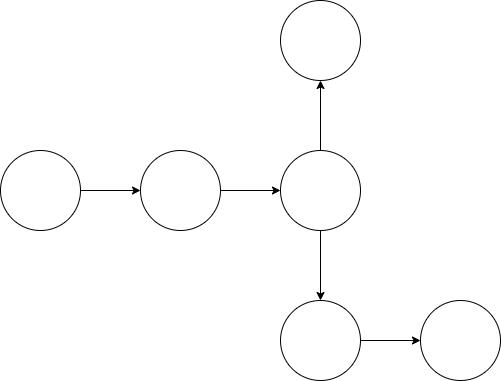
\includegraphics[width=5cm]{HelloWorldLevelSelect.png}
			\end{center}
		\end{figure}
		\item Puzzle Scene\\
		The Puzzle Scene will be the most involved portion of our prototype. Desired 
		mechanics are listed below by discipline:\\

		\textbf{UI:} The Puzzle UI will need to allow the player to perform the basic 
		puzzle solving operations. It should present the player with an instruction 
		set (\textit{Input, Output}) from which they may drag instructions into a solution 
		window. The Puzzle UI should present controls to allow the player to begin and 
		terminate the simulation of their solution. When the player's solution is being executed, 
		the UI should prohibit alterations to the solution window and display a program 
		counter to mark the current instruction being executed.\\

		\textbf{Level Design:} The level design of the Puzzle Scene will present all of the 
		static elements that will be present in every puzzle of our game. It will display an 
		input box with randomly generated contents, an output box that can accept objects 
		from the Actor, and a simple background plate.\\

		\textbf{Puzzle Logic:} Working in tandem with the level design, the puzzle scene's 
		logic system should be operational. Puzzle Logic is responsible for loading the scene 
		with the appropriate puzzle information. This includes a randomly generated input 
		box, the level prompt, an expected output, and the logic to read the output box 
		upon program completion to grade the player's solution.\\
    
		\textbf{Interpreter:} The Interpreter is the glue that binds the UI controls to the 
		Actor system. For this milestone, the Interpreter should be able to access and 
		process the player's solution stored in the solution window. When the player 
		starts the simulation, the Interpreter should process the instructions (ensuring 
		none are malformed) and make them available to the Actor upon request. 
		When the Actor requests an instruction, the interpreter will update its program 
		counter accordingly and report the counter's new position to the UI. The 
		Interpreter's PC calculation should be fully operational for the Input, Output, 
		and Unconditional Jump commands.\\

		\textbf{Actor:} For this milestone, the Actor should be able to query the Interpreter 
		for instructions to execute and interact with static level elements. Upon receiving an 
		input command, the Actor should move to the input box and remove at item. The 
		currently held item should be displayed on the Actor. Upon receiving an output 
		command, the Actor should move to the output box and deposit the currently 
		held item. If the Actor does not have an item in hand, it should report a fault to the 
		Interpreter so that simulation can be halted. If the Actor sees two input commands 
		back to back, it should discard its currently held item and attempt to take from the 
		input box again.\\
	\end{itemize}
\newpage
	\item Art\\
	For this milestone, programmer art placeholders are acceptable. However, the team should 
	have a plan in place to acquire quality art assets.
\end{itemize}

\subsection{Waterfall Method (Thursday, December 5th)}

\subsubsection*{Summary}
This milestone marks the deadline for Senior Design I documentation submission. This document 
must be complete, professionally bound, and delivered to HEC-345 by 1:00PM.

\subsubsection*{Deliverables}
As per the requirements of this course, our final design document will describe
all aspects of the project including:
\begin{enumerate}
	\item An Executive Summary\\
	The Executive Summary will give a high level overview about the purpose of the project 
	and how the project will fulfill that purpose. The Executive Summary should be written in 
	language accessible to non-technical professionals.
	\item A section detailing project significance\\
	This section should echo our Executive Summary in greater detail, with more specific language.
	\item A section describing our requirements\\
	This section should include an exhaustive list of our project's functional and non-functional requirements.
	\item A section detailing our game's design process\\
	This section should describe the team's efforts in discovering project requirements, and relate 
	the game mechanics chosen to the projects goals.
	\item A section detailing our game's technical design\\
	This section should describe the layout of the game's code systems. It should include 
	detailed technical discussions and diagrams to guide development.
	\item The project's milestones\\
	The milestones will be sets of requirements to ensure the project remains on track.
\end{enumerate}

\subsection{Open to Interpretation (Friday, January 10th)}

\subsubsection*{Summary}
``Open to Interpretation" will mark the project's first Alpha release. In this state, the game 
should be functional enough to place in front of a playtester with minor developer 
intervention. All basic game mechanics will be fully functional, and observing gameplay 
should produce relevant observations for the development team.

\subsubsection*{Deliverables}
This milestone’s deliverable is a stable Alpha release of our game. The requirements of the 
Alpha release are as follows:

\begin{itemize}
	\item Player experience\\
	The player experience should be polished enough to allow an individual with no 
	experience with our project to pick up and play it. All controls presented to the 
	player should work as expected, free of any noticeable bugs or glitches. Menus 
	should allow for proper flow between the game's scenes, and incomplete or 
	non-functional menus should be marked as such.

	Specifically, the player should be able to perform the following operations:
	\begin{enumerate}
		\item Launch the game from outside the Unity Editor.
		\item Start the game from the main menu, and enter the puzzle selection scene.
		\item Upon first run, only the first level of the game should be unlocked.
		\item Subsequent levels will only be unlocked after the player completes a puzzle.
		\begin{itemize}
			\item Exiting a puzzle without solving it will not unlock new puzzles
		\end{itemize}
		\item Puzzle unlocking will have an associated visual when returning to the level select screen.
		\begin{itemize}
			\item Player controls will be disabled and player focus should be drawn to the unlocked levels. (e.g. Camera zoom, simple animations, etc.)
		\end{itemize}
		\item After selecting a puzzle, the player should be transferred to the puzzle scene. The game should have at least two distinct levels.
		\item In the puzzle scene, the following mechanics should be operational.
		\begin{itemize}
			\item The instruction set pane shows only the subset of instructions chosen 
			to be available for that puzzle.
			\item Instructions can be dropped into the solution pane and manipulated in an intuitive way
			\item If the puzzle includes Memory Cards, the cards are displayed at the 
			bottom of the screen and are interactable.
			\item Move and Copy instructions are not usable until at least one 
			Memory card is in play.
			\item Memory Cards can be placed on, removed from, and re-ordered in 
			the play area.
			\item A Memory Card cannot be removed if it is referenced by an 
			instruction in the solution window. Instructions blocking card removal are 
			highlighted when the player's request fails.
			\item Computron is capable of interacting with the Inbox, Outbox, and registers.
		\end{itemize}
	\end{enumerate}
	\item Available Puzzles\\
	Puzzles 3, 4 of the tutorial sequence specified in Section~\textbf{\ref{section:tutorial}}.
	\item Available Mechanics
	\begin{itemize}
		\item Level Selection\\
		The level selection scene allows players to chose which puzzle they'd like to attempt. 
		Choosing a level should transfer the player to the Puzzle Scene with the relevant puzzle 
		data loaded. The player will be restricted in which puzzles are available, and have more unlocked as they successfully complete them.
		\item Basic instruction writing\\
		Player can click and drag the INPUT, OUTPUT, MOVETO, MOVEFROM, JUMP, and 
		JUMP IF NULL instructions into the instruction pane. Jump instructions allow player 
		to click-and-drag to set jump anchor.
		\item Basic Memory Card Manipulation\\
		Player is presented and can interact with a hand of memory cards on levels that require 
		them. Cards can be played, reorganized, and removed. MOVETO and MOVEFROM 
		instructions are active if and only if there is at least one Memory Card on the board.
		\item Basic Solution Grading\\
		After a player completes a puzzle, they are presented with a score sheet that provides 
		metrics on the par for:
		\begin{itemize}
			\item Instruction count
			\item Solution Runtime
			\item Memory Card cost
		\end{itemize}
		After they are done viewing this screen, they will be transferred back to the puzzle selection scene where they will see new levels unlock.
	\end{itemize}
\end{itemize}

\subsection{Tutorializing (Wednesday, February 12th)}

\subsubsection*{Summary}
``Tutorializing" will mark the Computron's second Alpha release. For this release, the tutorial 
system will be greatly expanded to allow for more hands-off playtesting.

\subsubsection*{Deliverables}
This milestone’s deliverable is another stable Alpha release of our game. The expected new 
features are listed below:

\begin{itemize}
	\item Available Puzzles\\
	Puzzles 1 through 9 of the tutorial sequence specified in Section~\textbf{\ref{section:tutorial}}.
	\item Available Mechanics
	\begin{itemize}
		\item Level Selection\\
		The level selection menu should meet the following requirements:
		\begin{itemize}
			\item Level selection menu supports a strong ordering of tutorial levels.
			\item Level selection menu allows for optional paths that do not impede player 
			progression
			\item The player's performance on puzzles (number of stars) should be recorded 
			and restored between play sessions.
			\item Advanced levels should be restricted from play until the player earns the 
			requisite number of points to unlock them.
		\end{itemize}
		\item Instruction Writing\\
		The puzzle writing and interpreting system should support the following instructions:
		\begin{itemize}
			\item INPUT
			\item OUTPUT
			\item JUMP
			\item JUMP IF NULL
			\item JUMP IF LESS
			\item JUMP IF GREATER
			\item MOVETO X
			\item MOVEFROM x
		\end{itemize}
		\item Memory Card Manipulation\\
		Player memory card interactions should be well polished. Players should find 
		playing and removing cards an intuitive part of the puzzle solving process. In 
		addition, the following cards should be operational:
		\begin{itemize}
			\item Register
			\item Stack
		\end{itemize}
	\end{itemize}
\end{itemize}

\subsection{Breaking Beta (Friday, February 28th)}

\subsubsection*{Summary}
``Breaking Beta" is Computron's first Beta release. At this point, the game's minimum 
viable product should be feature complete, leaving ample time to rework and refine 
mechanics based on intense playtesting.

\subsubsection*{Deliverables}
\begin{itemize}
	\item Available Puzzles\\
	Puzzles 1 through 12 of the tutorial sequence specified in Section~\textbf{\ref{section:tutorial}}.
	\item Available Mechanics
	\begin{itemize}
		\item Instruction Introductions\\
		Messaging should be added to attract the player's attention to new instructions 
		when they are made available. Upon first receipt of a new instruction, the User 
		Interface should display an interactive menu that allows players to unbox their 
		new command.
		\item Instruction Writing\\
		In game documentation of how instructions work is available from the puzzle scene.
		\item Memory Card Manipulation\\
		In game documentation of how a memory card works is available from the puzzle scene.
	\end{itemize}
\end{itemize}

\subsection{FIEA Playtest (Monday, March 2nd)}

\subsubsection*{Summary}
The team's advisor has offered to allow \textit{Computron} to be playtested by students 
at the Florida Interactive Entertainment Academy (FIEA). Playtesters from FIEA will span 
both technical and non-technical roles in game development, and will be able to offer 
valuable insights. It will be imperative to capture these insights, and use them to guide the 
final stages of the game's development.

\subsubsection*{Deliverables}
For this playtest, the team should be able to present a high quality build of the game. 
Fielding a high quality demo will be very important in allowing the team to gather effective 
observations from the playtesters. The team should arrive to the playtest with:
\begin{enumerate}
	\item A stable build of the game.
	\item A set of exit survey questions to track player experience.
	\item Several computers capable of playing the game to allow increased playtesting 
	bandwidth.
\end{enumerate}

After the playtest, the team should compile player feedback and evaluate which parts 
of the game will need more attention.

\subsection{Quick Math (Friday, March 20th)}

\subsubsection*{Summary}
``Quick Math" will be the second Beta release of Computron. It will feature an expanded 
instruction set and new puzzles that make use of mathematical principles. 

\subsubsection*{Deliverables}
\begin{itemize}
	\item New Instructions\\
	Computron should support four brand new instructions:
	\begin{itemize}
		\item ADD X
		\item SUBTRACT X
		\item BUMP++
		\item BUMP-\--
	\end{itemize}
	\item New Puzzles\\
	This release should feature three new puzzles that exercise the new problem spaces 
	made accessible by the expanded instruction set:
	\begin{enumerate}
	\item Adding Machine\\
	This puzzle should introduce players to the mechanics of the new ADD instruction. 
	Puzzle should ask players to add pairs of numbers in the input and output their sum.
	\item Subractinator\\
	This puzzle should introduce players to the mechanics of the new SUBTRACT instruction. 
	Puzzle should ask players to subtract pairs of numbers in the input and output their difference.
	\item Hexiplier\\
	This puzzle should show players an application of the new ADD instruction. For each number 
	in the input, the puzzle should expect that number times 6 as output.
	\end{enumerate}
\end{itemize}

\subsection{Release Candidate (Friday, April 10th)}

\subsubsection*{Summary}
Nearing the end of our project, milestone requirements will largely be determined by 
the state of the game and the results of playtests. For this milestone, the team should 
have most of the concerns raised from the FIEA playtest fully remedied.

\subsubsection*{Deliverables}
A fun release candidate of \textit{Computron}.

\subsection{Mission Accomplished (Wednesday, April 15th)}

\subsubsection*{Summary}
``Mission Accomplished" marks the final release of \textit{Computron}. The project should 
be in a state that accomplishes the goals set forth in this document.

\subsubsection*{Deliverables}
A game the team is proud of.